\chapter{\IfLanguageName{dutch}{Opstellingen}{Opstellingen}}
\label{ch:opstellingen}

In dit hoofdstuk zullen de 12 verschillende opstellingen die in het volgende hoofdstuk onderzocht worden opgelijst worden, samen met een ruwe schets van hoe deze opstelling eruit zal zien en een korte uitleg over hoe deze opstelling theoretisch zou moeten werken en de voor- en nadelen ervan.
De verschillende opstellingen zullen onderverdeeld worden per categorie, allereerst op technologie, maar verder ook volgens het statische of het dynamische principe. 
Deze laatste onderverdeling houd als volgt in:
\begin{itemize}
	\item \underline{Statisch}:
	In een statische opstelling wordt elk voorwerp gekenmerkt door 1 RFID Tag of BLE beacon, en de locatie waarop deze zich bevind wordt gekenmerkt door een bepaald aantal readers (RFID-antennes of IoT Gateways), die de signalen van deze voorwerpen opvangen. Aan de hand van deze data wordt de locatie idealiter bekend.
	\item \underline{Dynamisch}:
	Bij een dynamische opstelling worden zowel de voorwerpen als de locaties gedefinieerd door RFID tags of BLE beacons. Hierbij is het concept dat er met de readers (RFID-antennes of IoT Gateways) wordt rondgegaan in het gebouw. De info die hieruit vloeit zal verder geaggregeerd worden en daaruit zullen de locaties van de voorwerpen bepaald worden. Dit systeem is minder real-time dan een statische opstelling, maar het is kostendrukkend aangezien een reader veel meer kost dan een tag of beacon, dus als hun aantal geminimaliseerd kan worden is dit voordelig.
	In theorie kunnen deze readers overal rondgaan, welke voor een RFID opstelling ook zo zal zijn. Echter is er, in samenspraak met Aucxis en het in beschouwing nemen van hun noden, beslist dat de IoT Gateways voor de BLE scenario's enkel in de gang tussen de locaties zullen rondgaan.
\end{itemize}

\subsubsection{De Illustratie}
\begin{minipage}{0.65\textwidth}
Elk van volgende opstellingen zal gebruik maken van een bijhorende figuur, gebaseerd op degene bijgevoegd hier. Dit is een schematische weergave van een systeem dat opgebouwd is volgens de te onderzoeken opstelling, ze heeft als doel hulp te bieden bij het begrijpen van hoe de opstelling en de definiëring van locaties eruit ziet, maar is niet noodzakelijk de testopstelling tijdens het onderzoek. Ook is hier elke logische locatie een kamer, maar dit is in praktijk niet noodzakelijk het geval (Een magazijn kan bv. opgedeeld zijn in meerdere zones zonder muren). Op volgende voorbeeldfiguur is de opbouw van de voorbeeldschets te zien, ze bestaat uit 5 locaties (weergegeven in kleur), en een gang (weergegeven in grijs). De gang is geen locatie, en is de plek waar doorgelopen zal worden met de readers bij een dynamische BLE opstelling.
\end{minipage}
\hfill
\begin{minipage}{0.30\textwidth}
	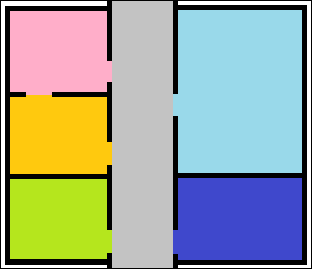
\includegraphics[width=\linewidth]{layout_alg}
\end{minipage}

\section[RFID]{De RFID opstellingen}
\label{ch:rfid}

\subsection{Statisch}

\subsubsection{1 antenne aan deurlijst}
\begin{minipage}{0.65\textwidth}
Deze opstelling is de eenvoudigste en 1 van de opstellingen die momenteel wordt gebruikt door Aucxis, ze is voornamelijk opgenomen in dit onderzoek als referentie. Het concept bij deze opstelling is dat aan elke deurlijst 1 RFID antenne hangt. Als er een tag voorbij de antenne gaat registreert deze dit en weten we dar er een beweging heeft plaatsgevonden. Of deze in of uit de locatie is kan niet uit deze data alleen afgeleid worden, dit kan enkel in combinatie met de informatie wat zijn locatie was voor de verplaatsing. Dit is een nadeel aan deze opstelling.
\end{minipage}
\hfill
\begin{minipage}{0.30\textwidth}
	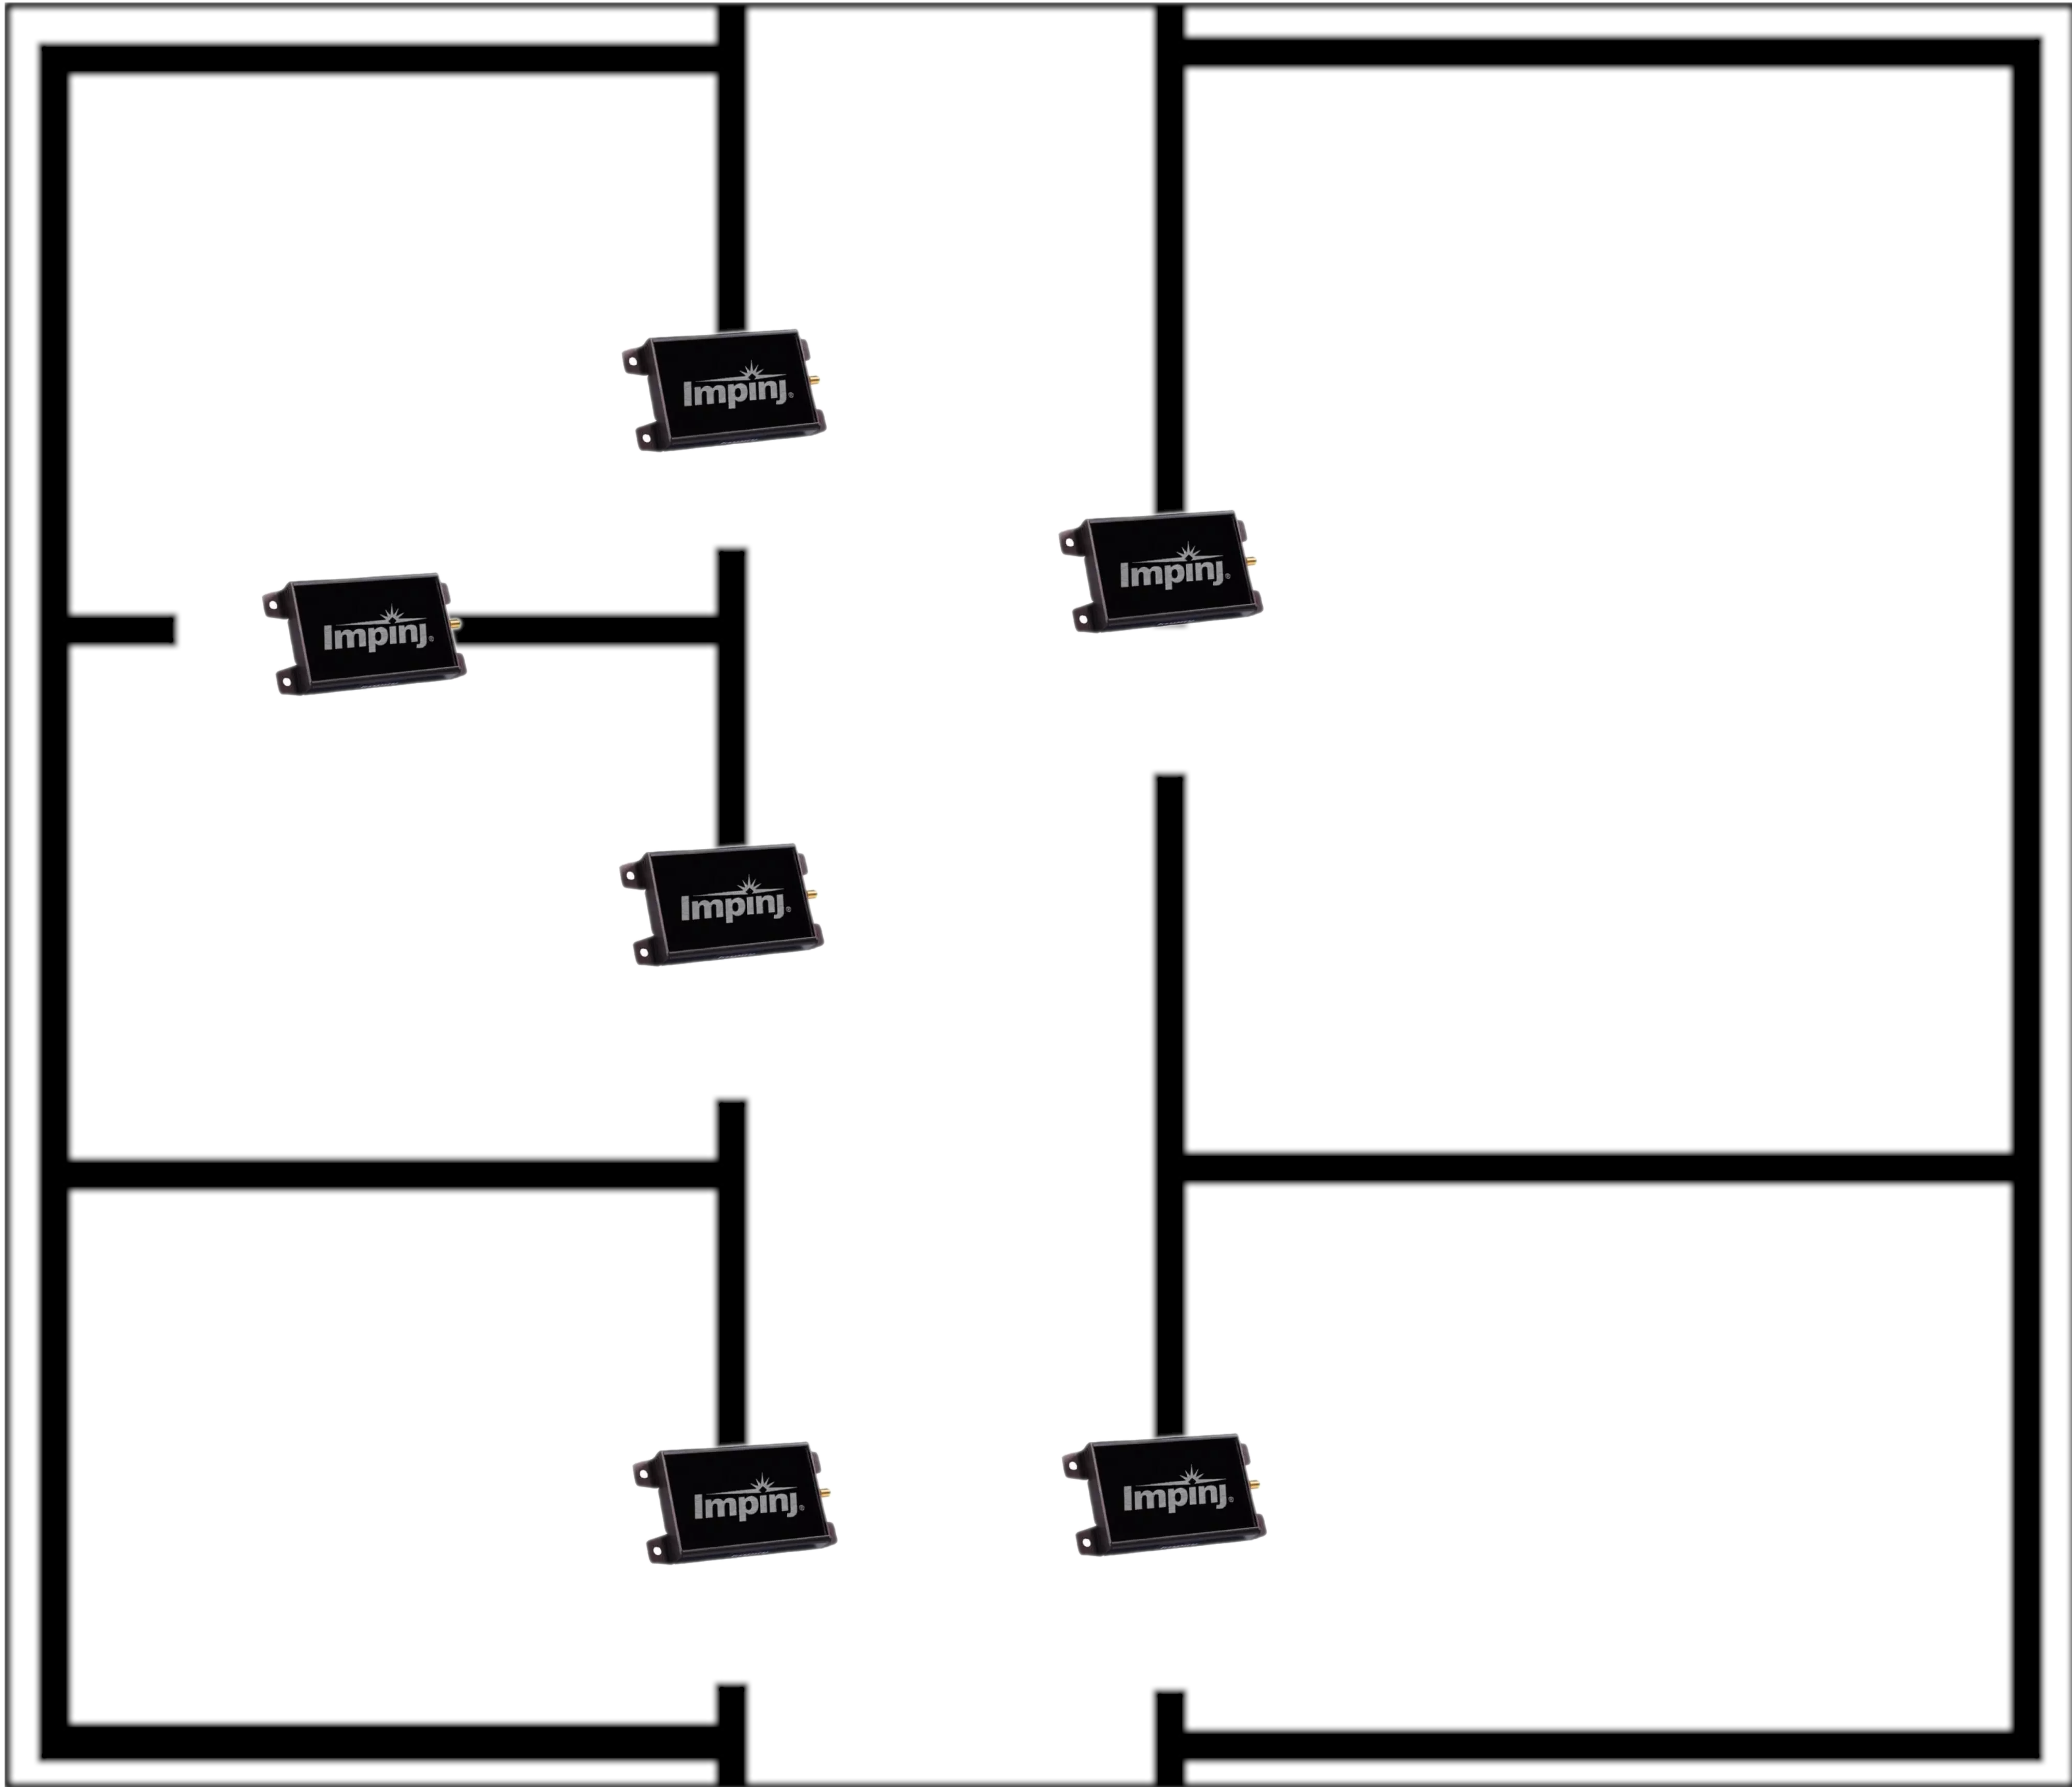
\includegraphics[width=\linewidth]{rfid_static_1}
\end{minipage}

\subsubsection{2 antenne aan deurlijst}
\begin{minipage}{0.65\textwidth}
Dit is ook 1 van de opstellingen die momenteel wordt gebruikt door Aucxis en dus ook voornamelijk een referentiepunt. Het principe is ongeveer hetzelfde als bij de vorige opstelling, echter is hier het voordeel dat de richting van de verplaatsing wel bekend is aan de hand van het tijdsverschil tussen de detecties van de tag. In dit opzicht is het dus beter dan de vorige opstelling, maar is uiteraard duurder door de hogere aantallen benodigde antennes. 
\end{minipage}
\hfill
\begin{minipage}{0.30\textwidth}
	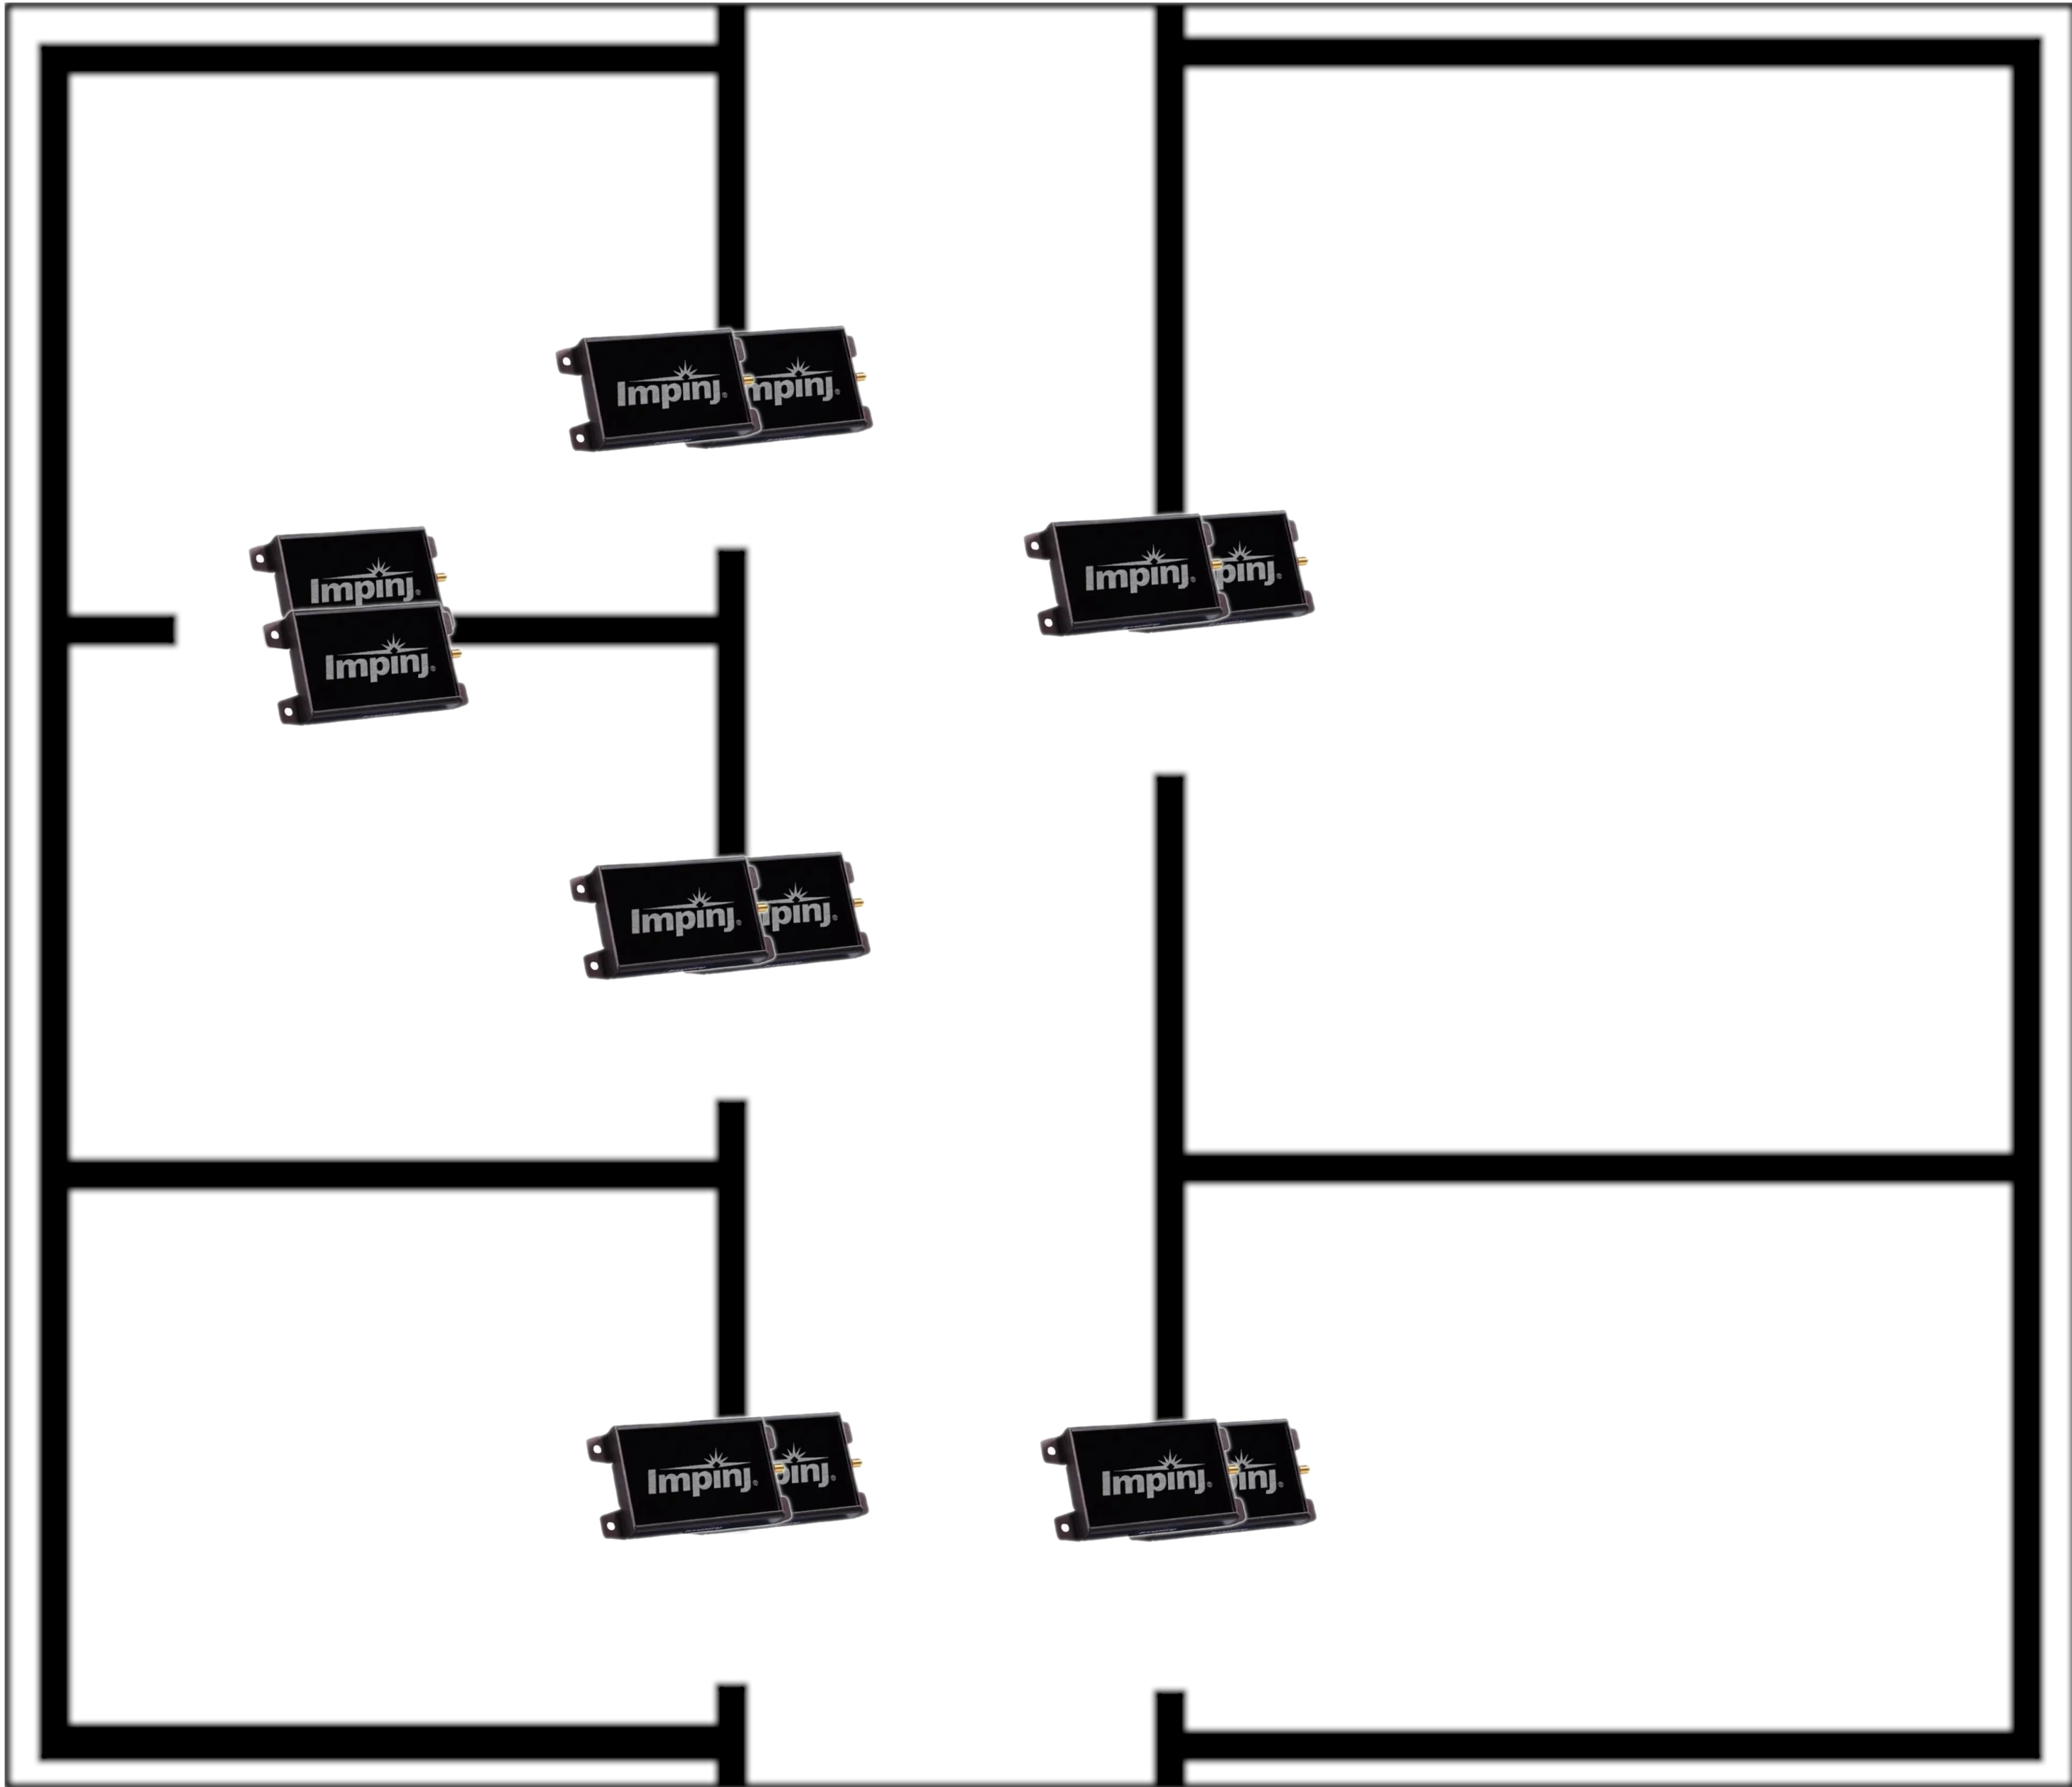
\includegraphics[width=\linewidth]{rfid_static_2}
\end{minipage}

\subsubsection{1 antenne tegenover deur}
\begin{minipage}{0.65\textwidth}
Bij deze opstelling wordt een RFID antenne tegenover de deur geplaatst, het idee hierachter is het feit dat, aangezien de RSSI afhankelijk is van de afstand tussen de antenne en de tag, het in theorie zichtbaar is aan de verandering in RSSI in welke richting de tag gaat. Ook geeft de antenne een doppler waarde mee, welke in theorie ook veranderd naargelang de richting. Als dit in praktijk blijkt te werken wilt dit zeggen dat er richtingsdetectie mogelijk is met 1 antenne, waardoor het sowieso al beter is dan de vorige 2 opstellingen. Nadeel is wel dat de kamer niet te breed mag zijn zodat de antenne ook tegenover de deur kan worden gemonteerd.
\end{minipage}
\hfill
\begin{minipage}{0.30\textwidth}
	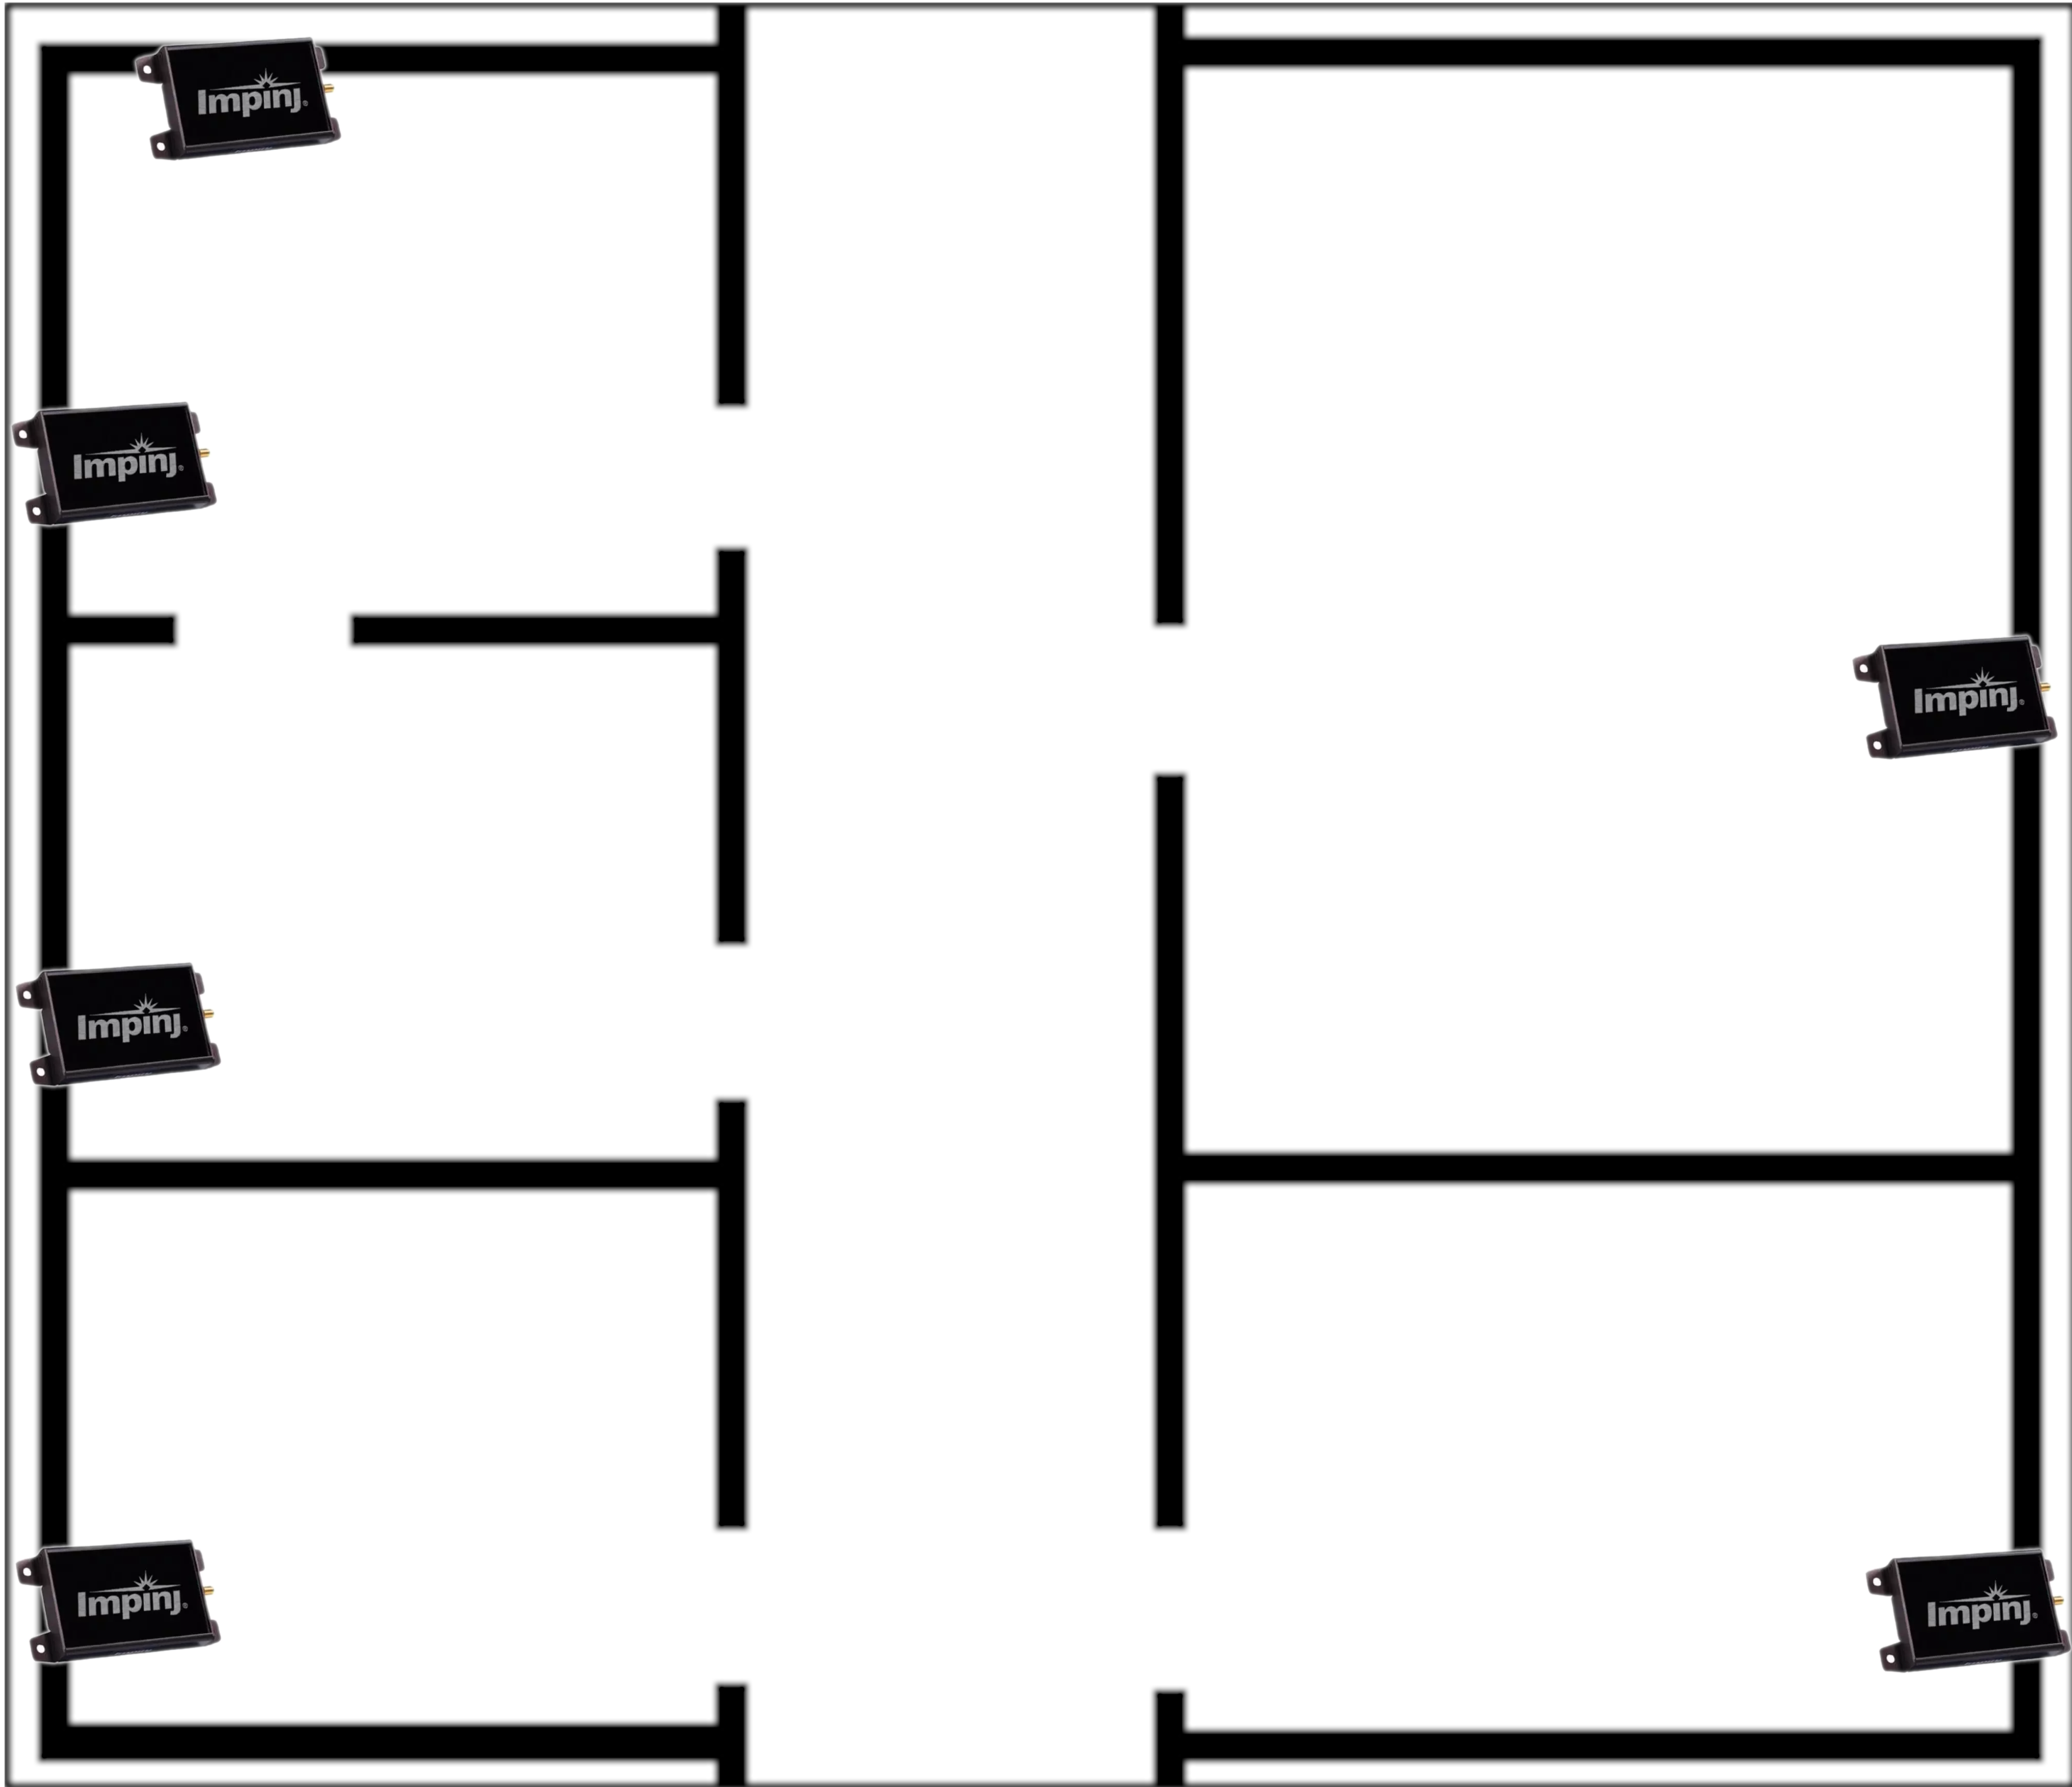
\includegraphics[width=\linewidth]{rfid_static_3}
\end{minipage}
\subsection{Dynamisch}

\subsubsection{1 tag aan deurlijst}
\begin{minipage}{0.65\textwidth}
Hier hangt er een RFID-tag aan de deurlijst (analoog aan de antenne bij de eerste statische opstelling). Als de antenne passeert aan de deur weet het aggregatieprogramma in theorie dat alle tags tussen nu en het passeren van deze of een andere locatie RFID-tag tot deze locatie behoren.
\end{minipage}
\hfill
\begin{minipage}{0.30\textwidth}
	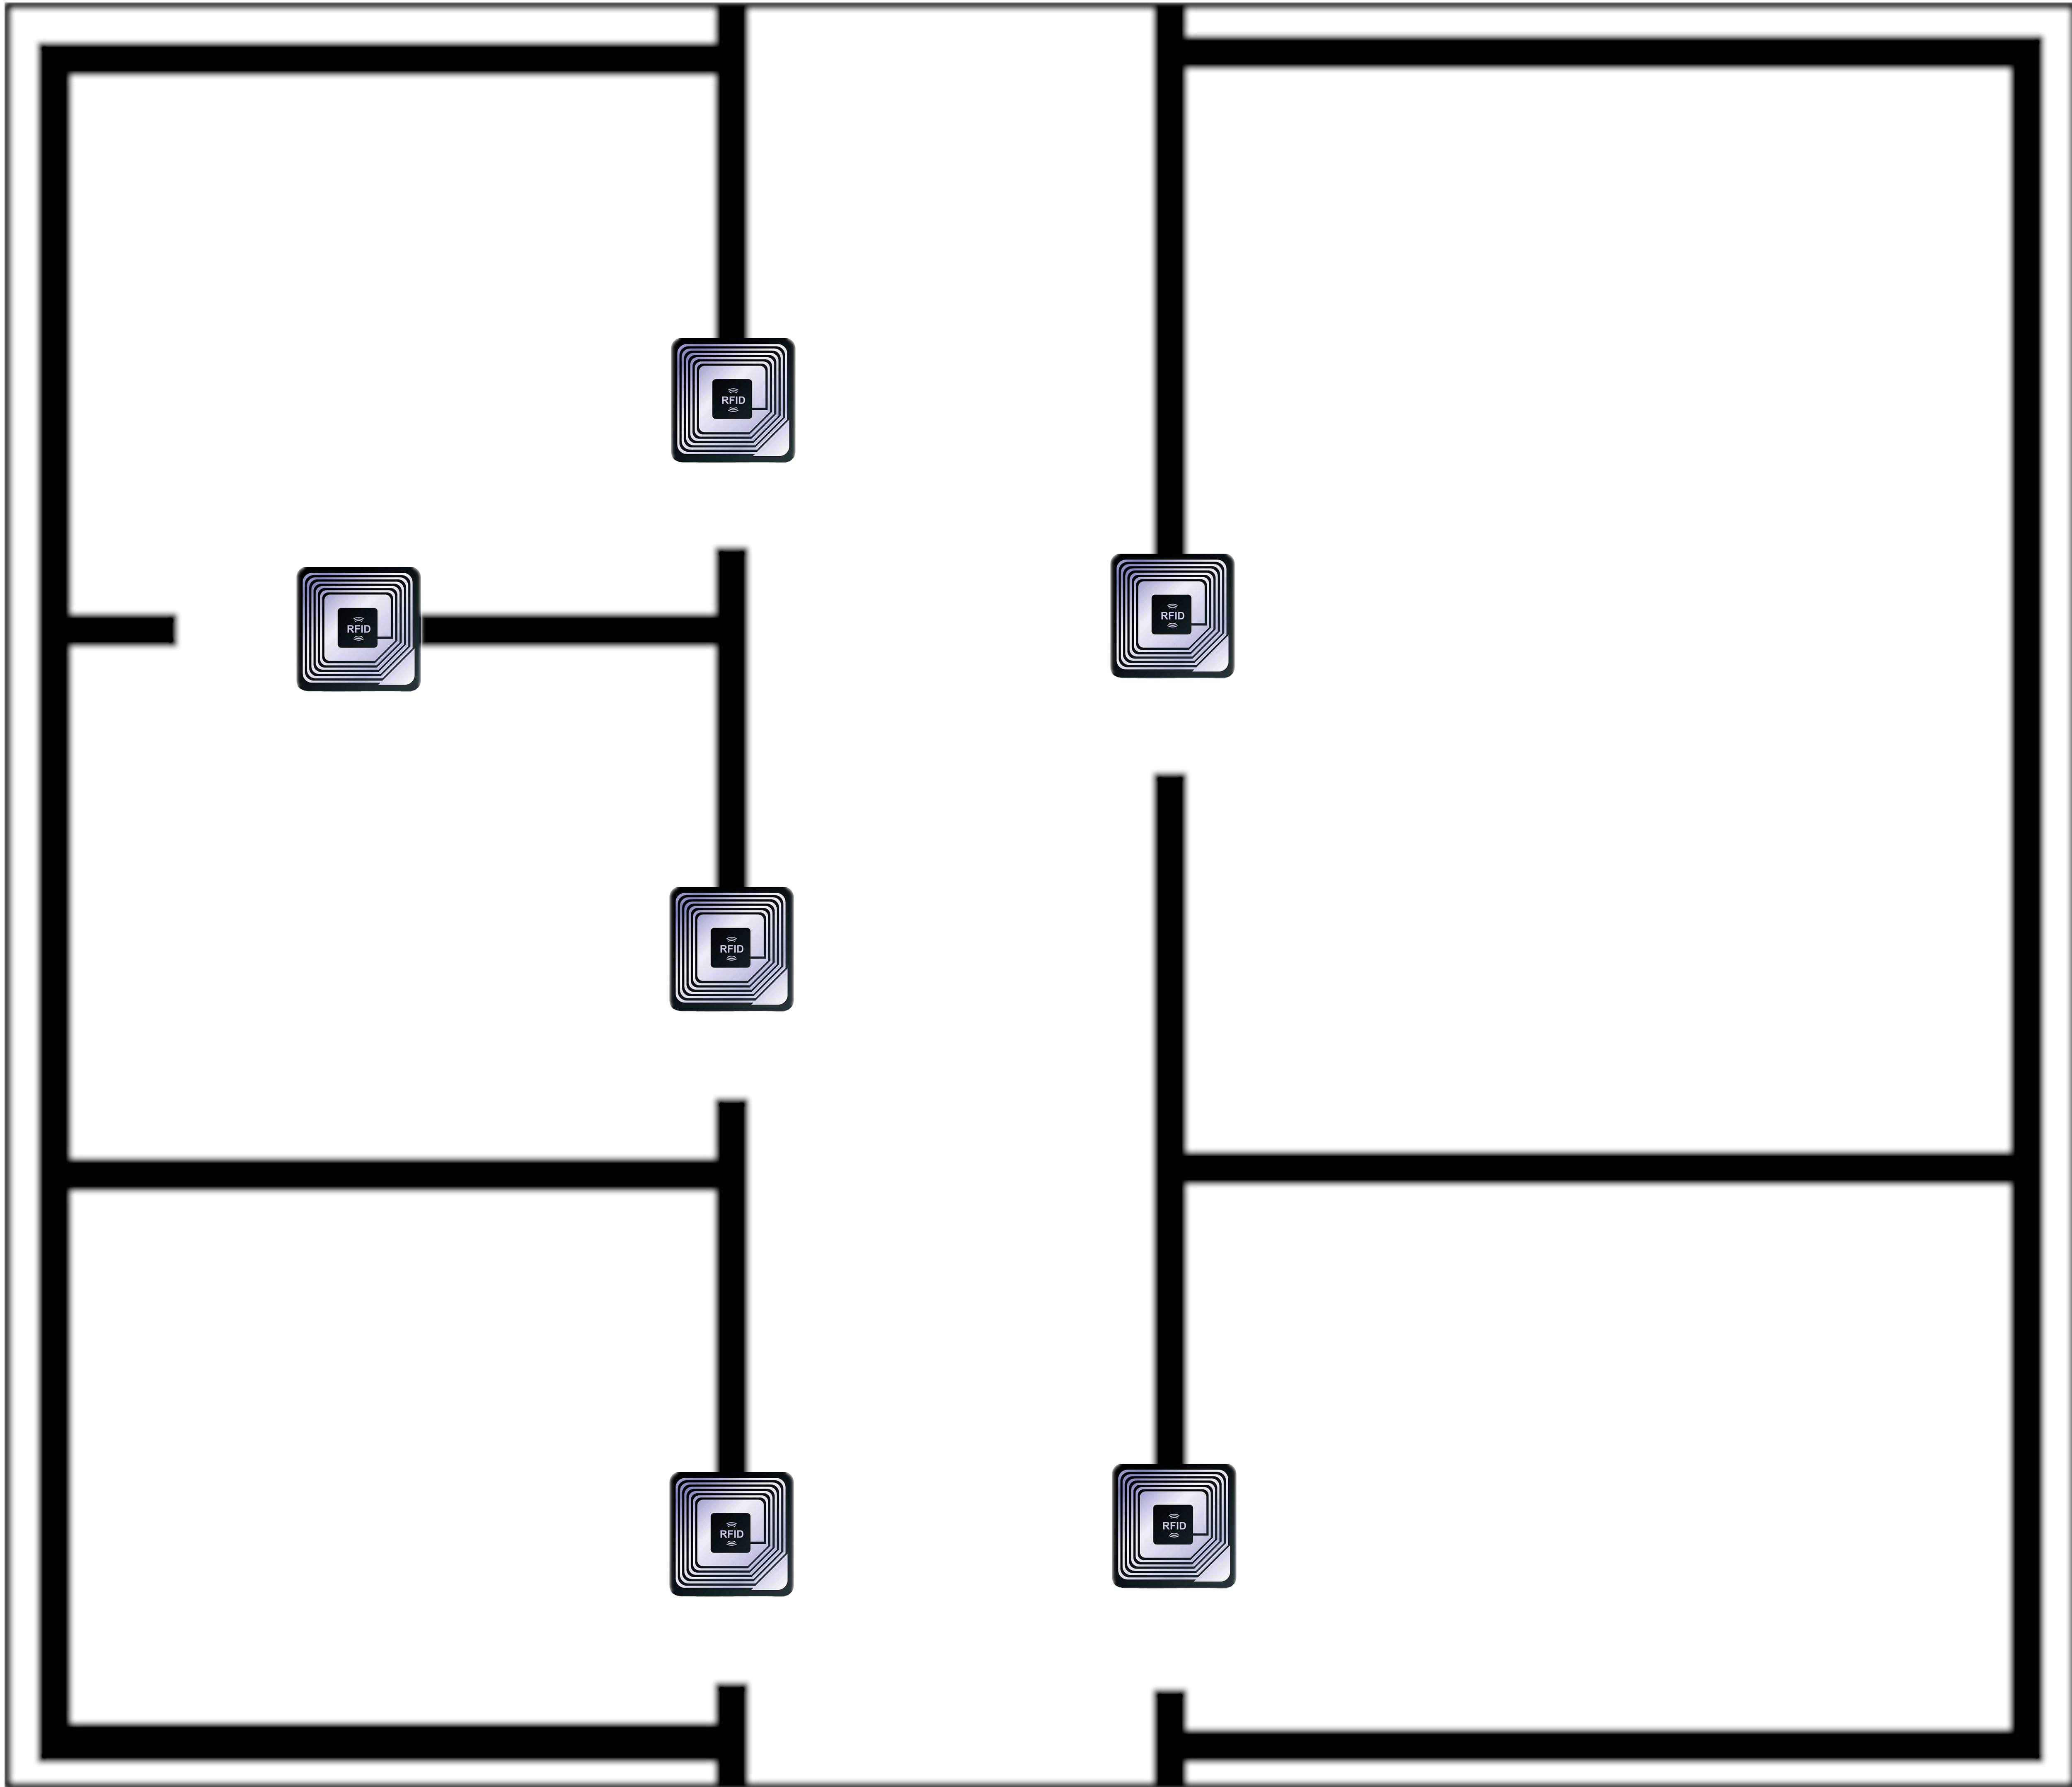
\includegraphics[width=\linewidth]{rfid_dynamic_1}
\end{minipage}

In theorie is het ook mogelijk de 2 andere statische scenario's een dynamische variant te geven, echter valt hun voordeel van richtingbepalend zijn weg hierbij aangezien de richting niet meer relevant is bij dynamisch. Deze worden dus buiten beschouwing gelaten.

\section[BLE]{De BLE opstellingen}
\label{ch:ble}

\subsection{Statisch}

\subsubsection{1 gateway per locatie}
\begin{minipage}{0.65\textwidth}
Deze opstelling is de eenvoudigste en meest intuïtieve van de BLE opstellingen. Elke locatie komt overeen met 1 IoT Gateway, die gepositioneerd wordt ongeveer in het middelpunt van de locatie. Het idee hierachter is dat de Gateway waar de beacon het dichtste bij is (de beste RSSI heeft), hoogstwaarschijnlijk de locatie is waar het voorwerp zich bevind. Dit is echter niet 100\% correct, en deze onnauwkeurigheid zal enkel maar groeien als de gateways/locaties onevenredig verdeeld zijn over de oppervlakte van het gebouw. 
\end{minipage}
\hfill
\begin{minipage}{0.30\textwidth}
	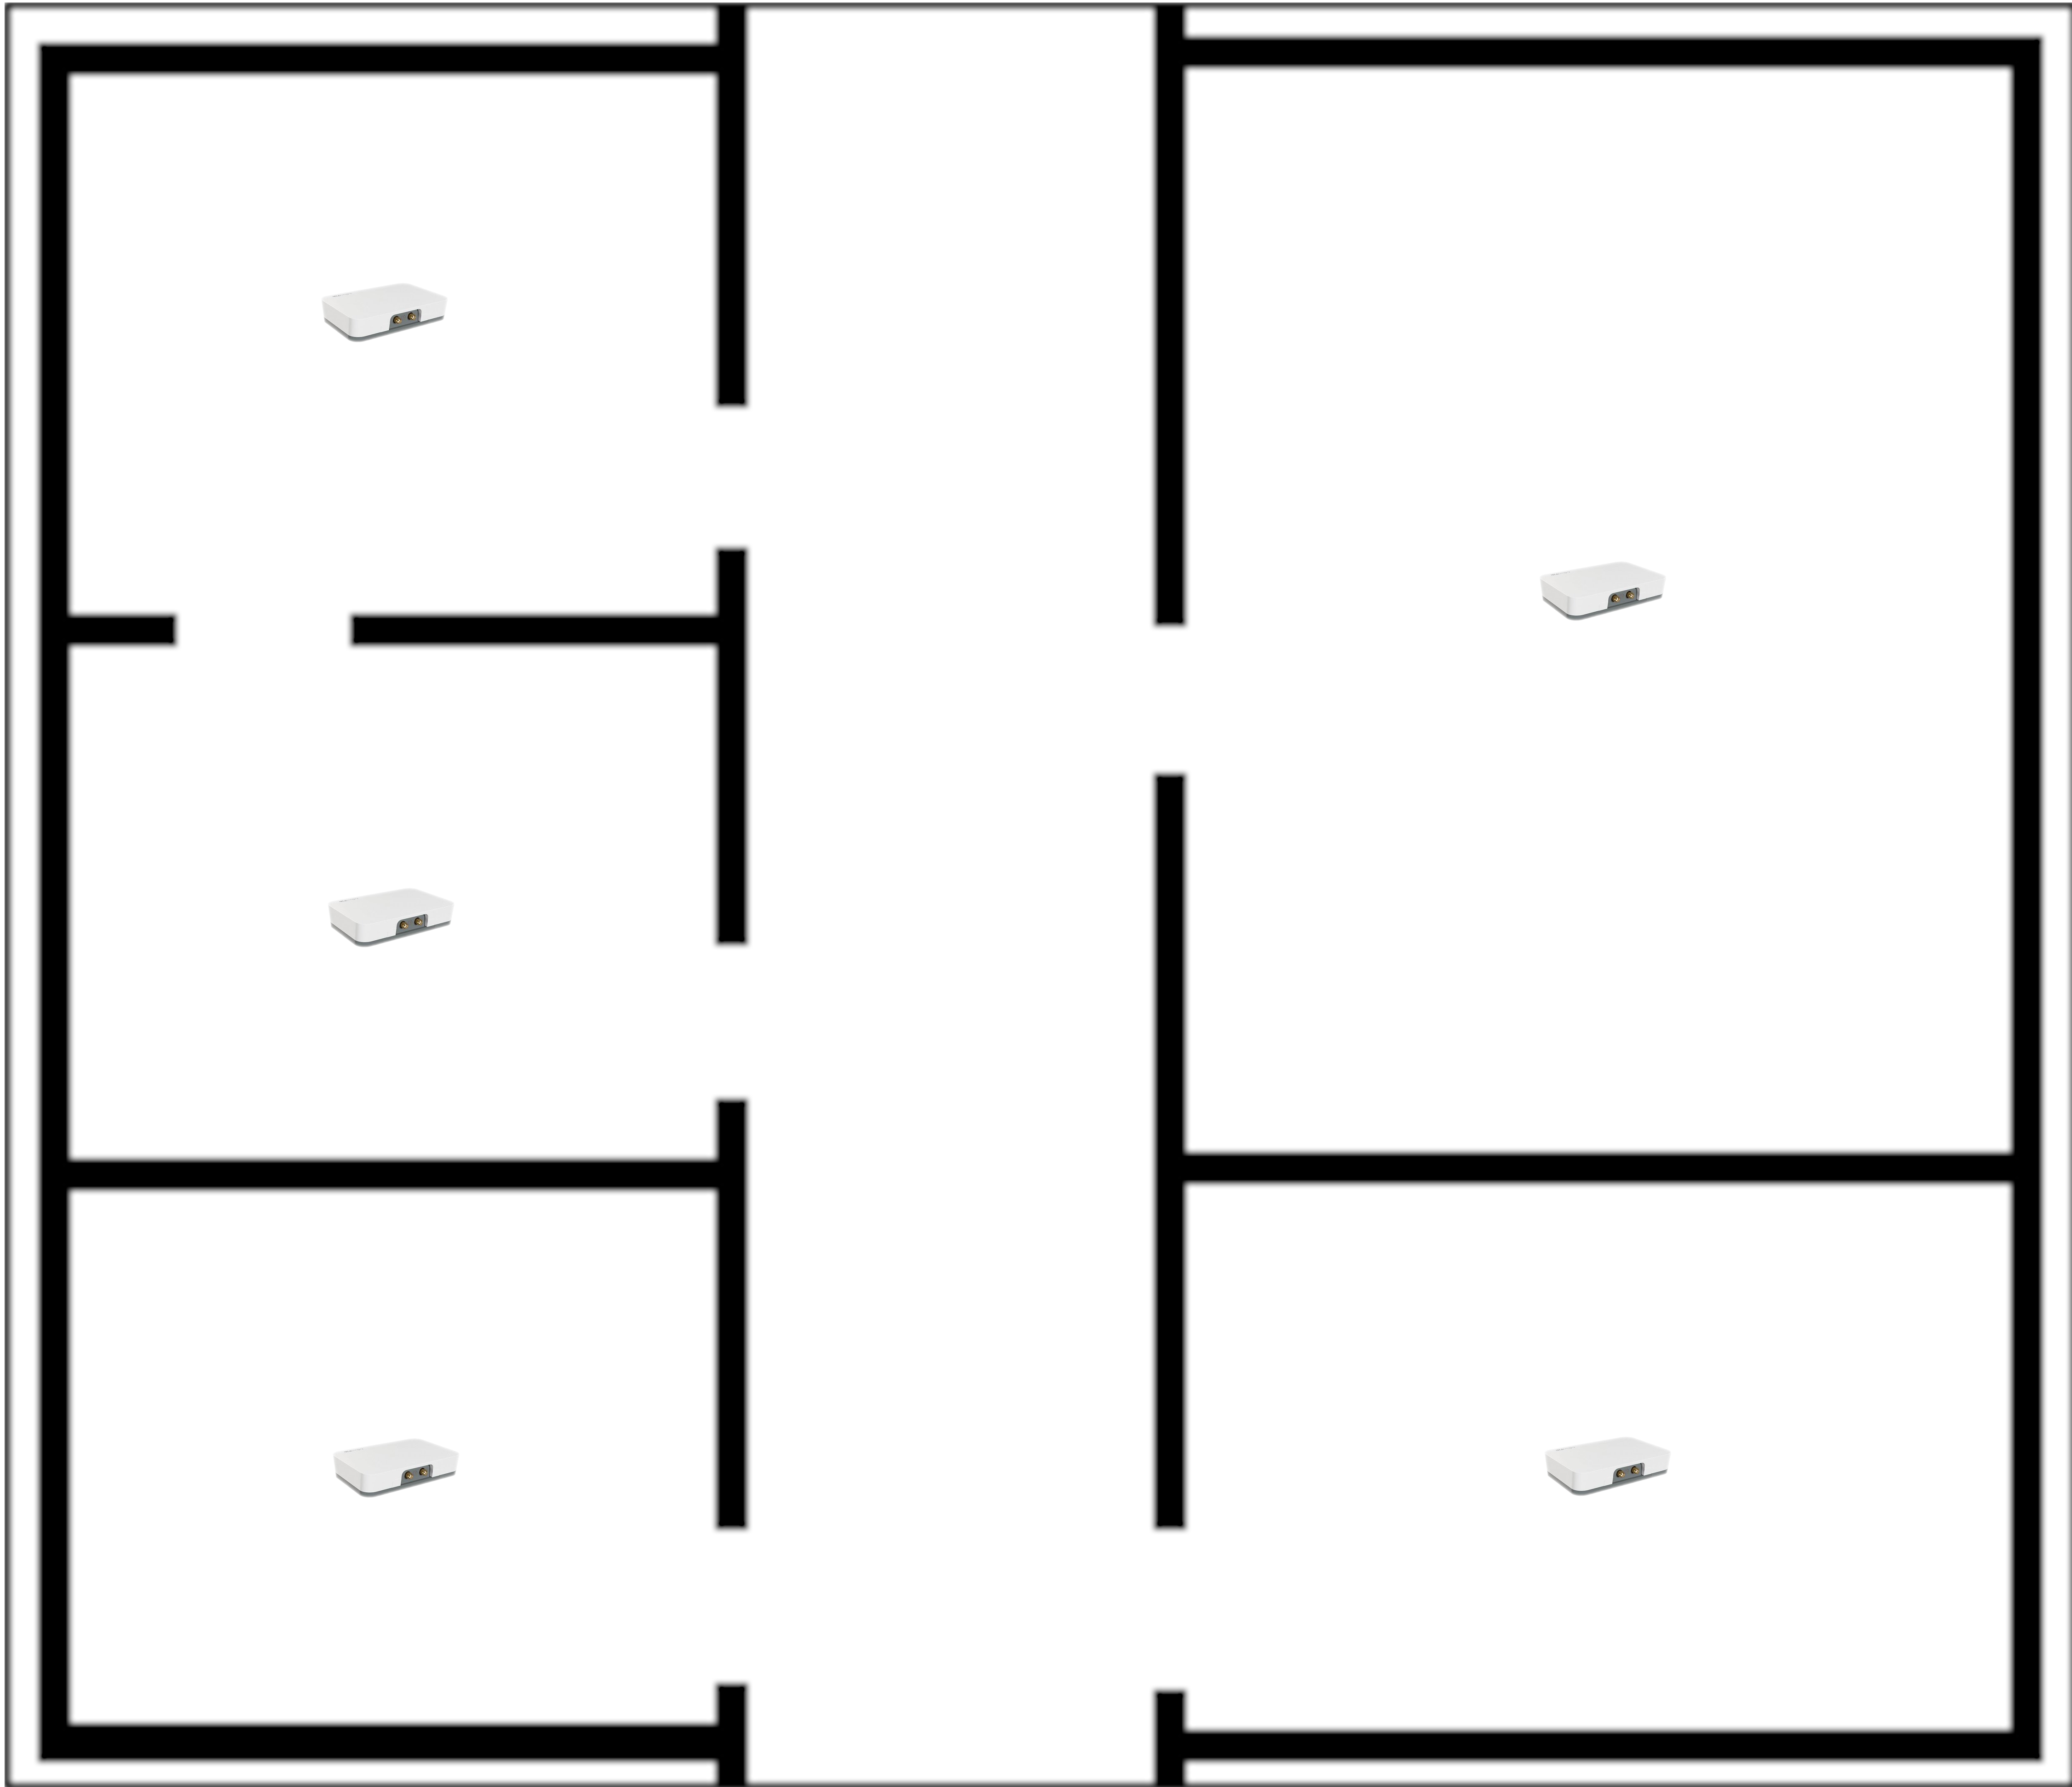
\includegraphics[width=\linewidth]{ble_statisch_1}
\end{minipage}

\subsubsection{Meerdere gateways per locatie}
\begin{minipage}{0.65\textwidth}
In deze opstelling wordt een locatie gedefinieerd door meer dan 1 gateway, nl. een gateway per hoek van de locatie, zodat de locatie wordt omringd door een kader van gateways. Hiermee kan in theorie zeer gedetailleerd worden afgeleid waar de beacon zich bevind, maar de kost voor de opstelling vliegt vrij snel de hoogte in als er veel locaties zijn. Wel kunnen gedeelde hoeken van locaties door een gedeelde beacon worden bezet.
\end{minipage}
\hfill
\begin{minipage}{0.30\textwidth}
	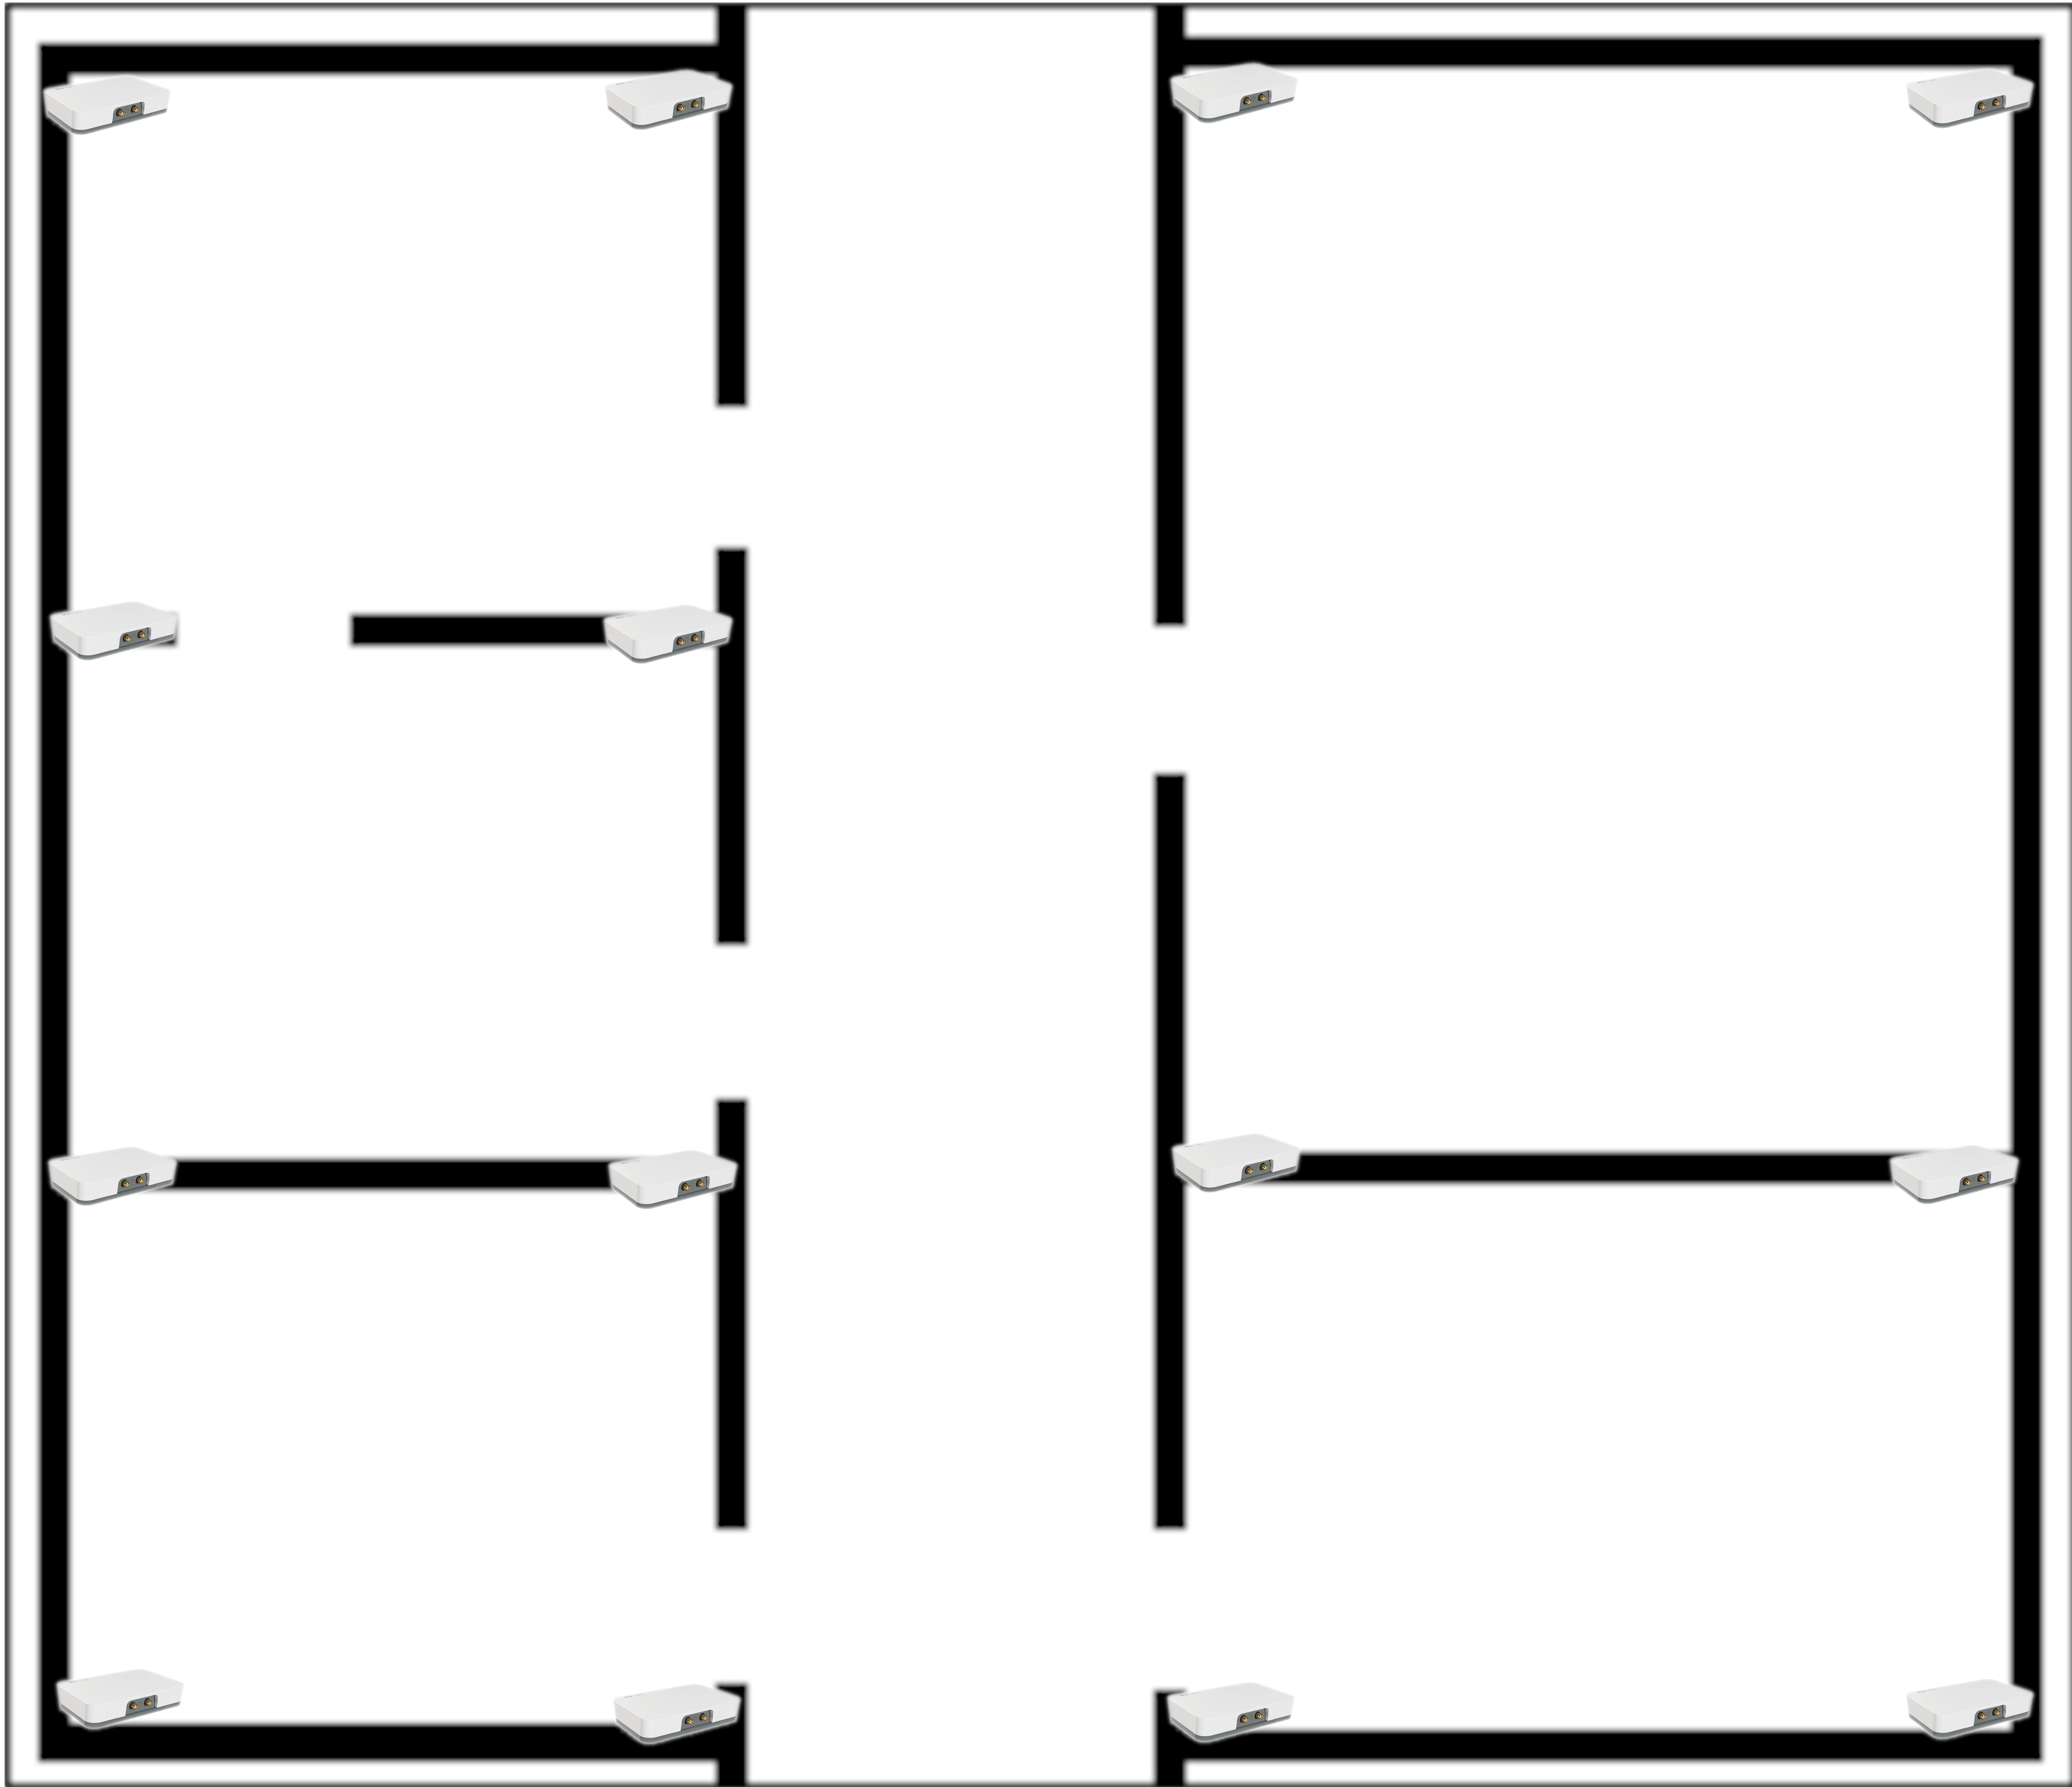
\includegraphics[width=\linewidth]{ble_statisch_2}
\end{minipage}

\subsubsection{Rasteropstelling}
\begin{minipage}{0.65\textwidth}
Deze opstelling bestaat uit een raster welke volledig het gebouw omvat. Als de locaties van deze gateways bekend zijn kan via trigonometrie en de gemeten RSSI waardes berekend worden waar de voorwerpen zich bevinden, wat dan gelinkt kan worden aan een locatie. Dit is vrij precies en schaalt goed, maar nadelig is wel dat de locaties volledig gespecificeerd en bijgehouden moeten worden want er kan niet enkel op data van de gateways worden afgegaan om de locatie te bepalen aangezien de gateways en de locaties niks meer met elkaar te maken hebben.
\end{minipage}
\hfill
\begin{minipage}{0.30\textwidth}
	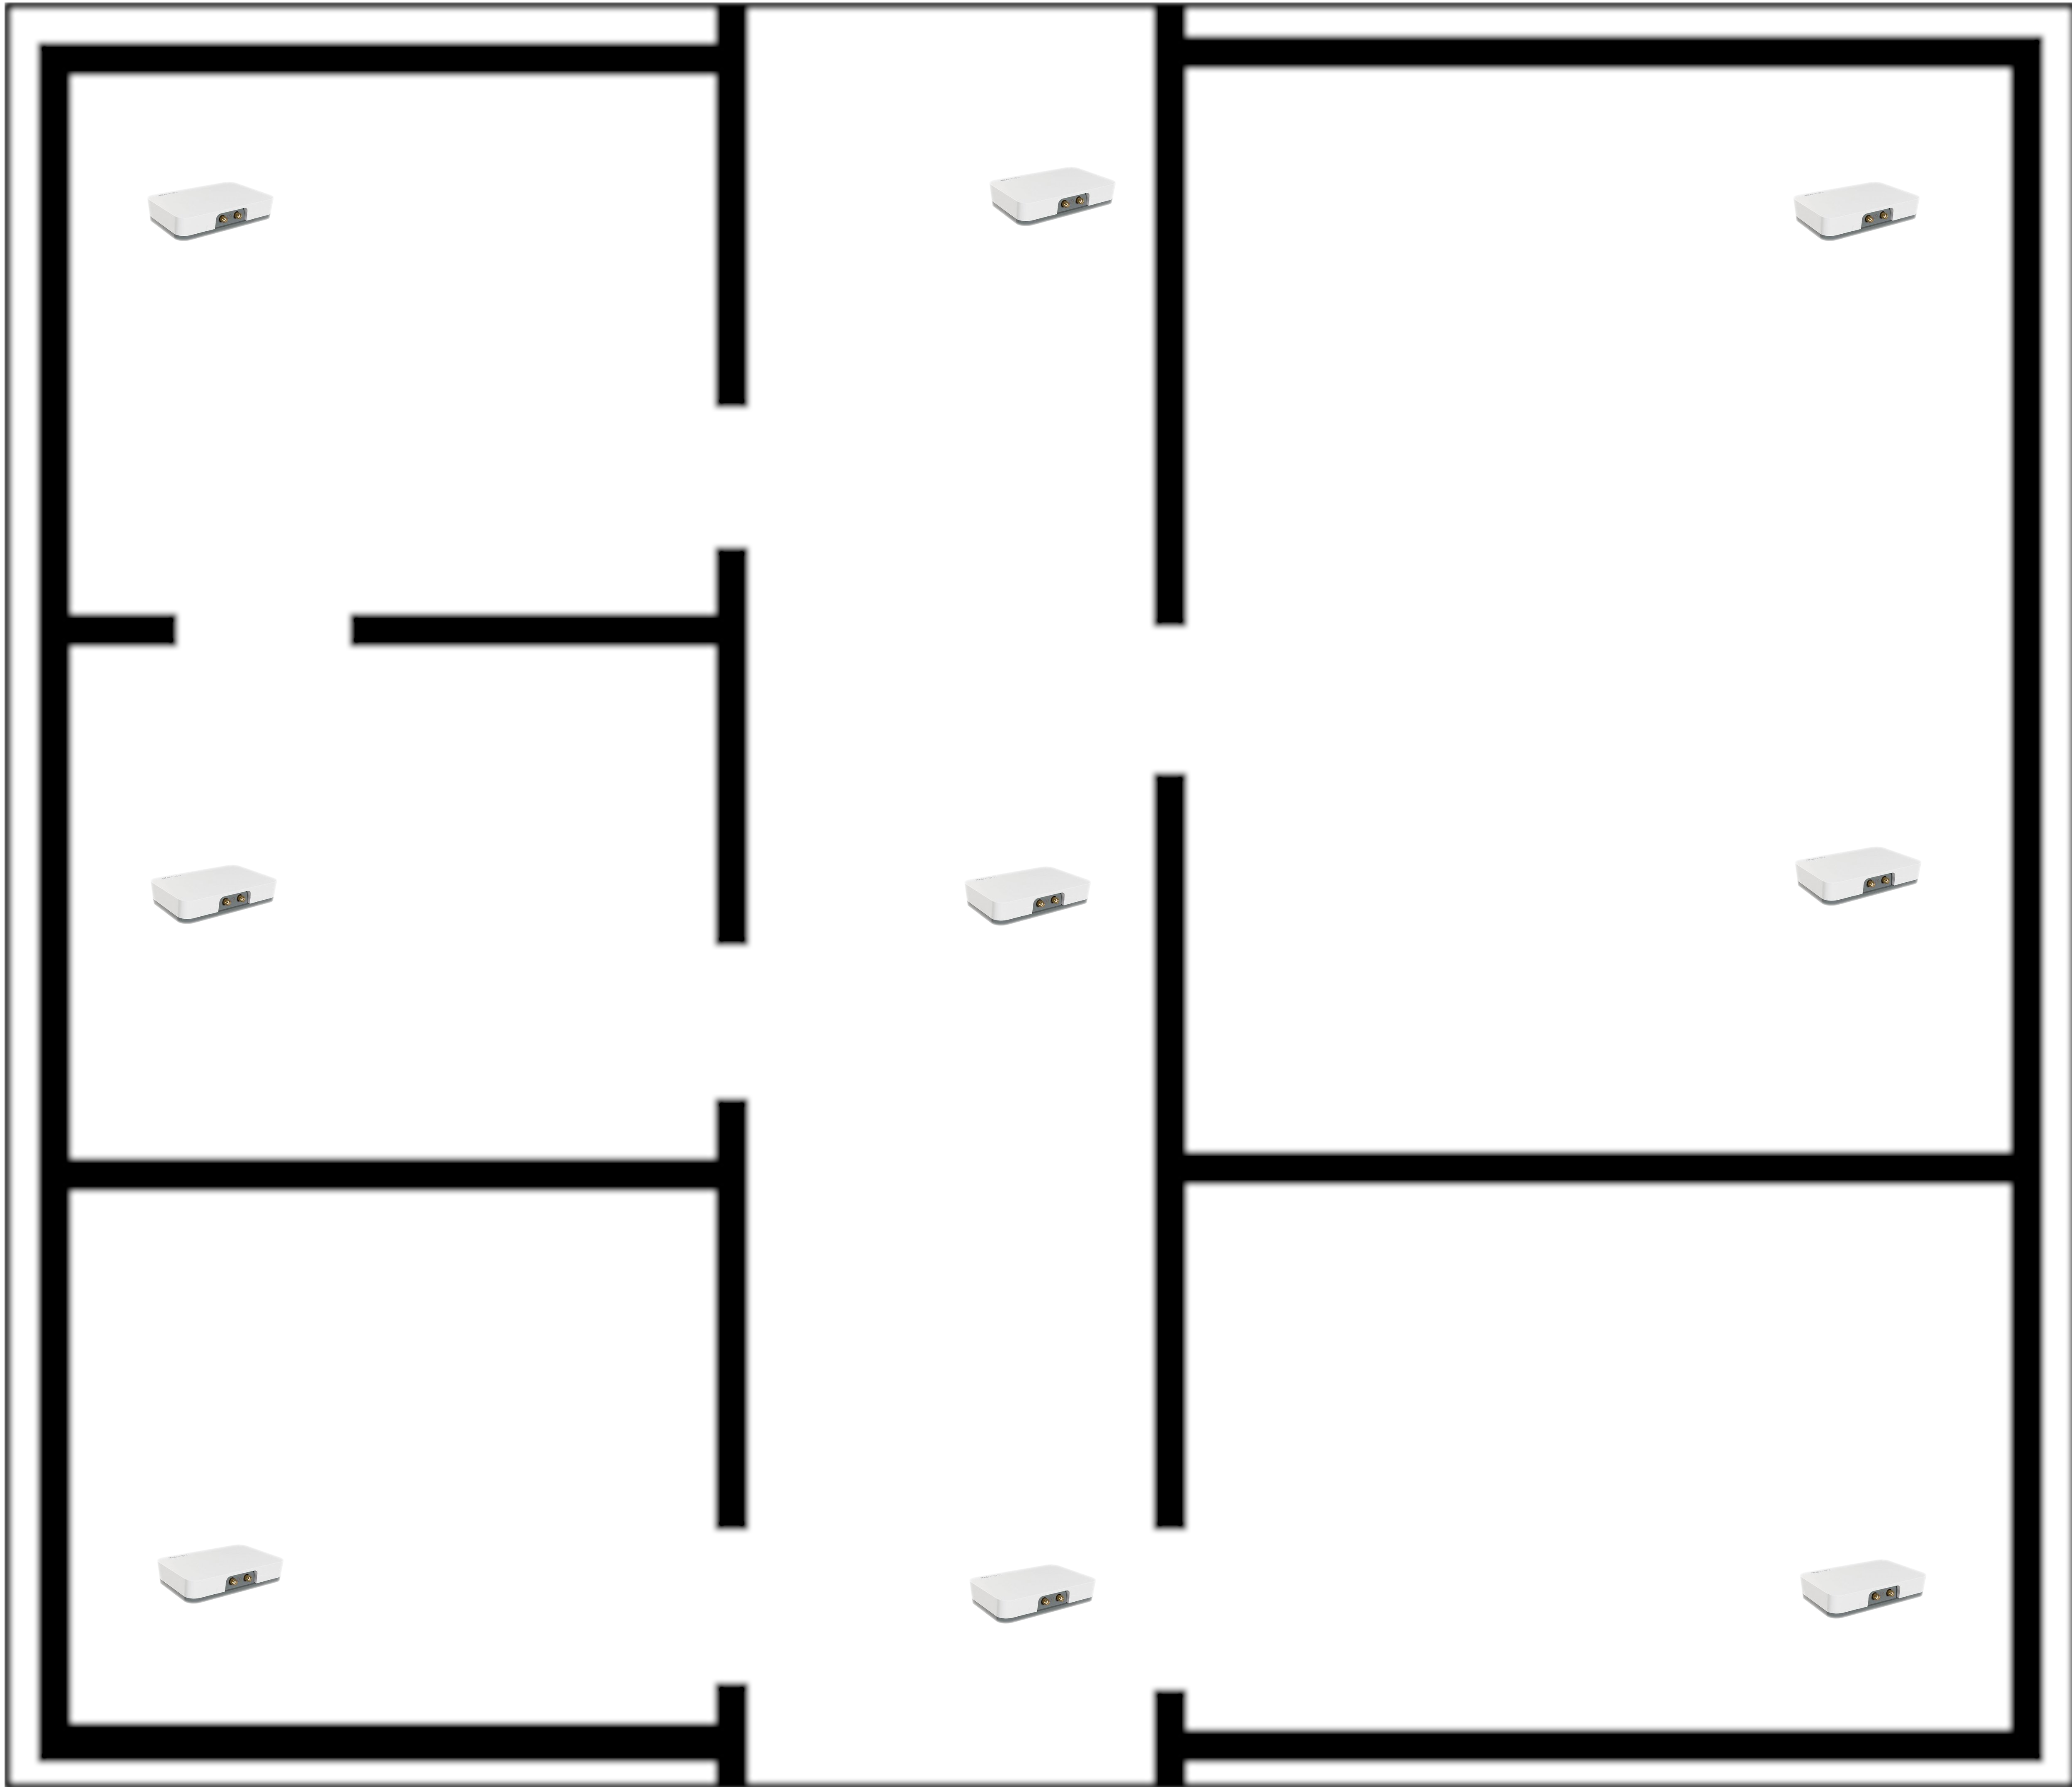
\includegraphics[width=\linewidth]{ble_statisch_3}
\end{minipage}


\subsection{Dynamisch}

\subsubsection{1 beacon per locatie, midden van kamer}
%TODO

\subsubsection{1 beacon per locatie, aan deur}
%TODO

\subsubsection{< 1 beacon per locatie}
%TODO

\subsubsection{> 1 beacon per locatie}
%TODO

\subsubsection{beacons op intervallen in de gang}
%TODO